Nedenfor ses, hvordan FlexPMS håndterer de usecases, som påvirker FlexPMS.

\subsubsection{Start manuel vanding}

Når manuel vanding startes for et kar, så skal alle ventiler, som sidder på sensor Ø'er, der er koblet til karret, åbnes. Derefter startes pumpen, som pumper vand ud til Ø'erne. Herefter registreres status i databasen.

\begin{figure}[H]
	\centering
	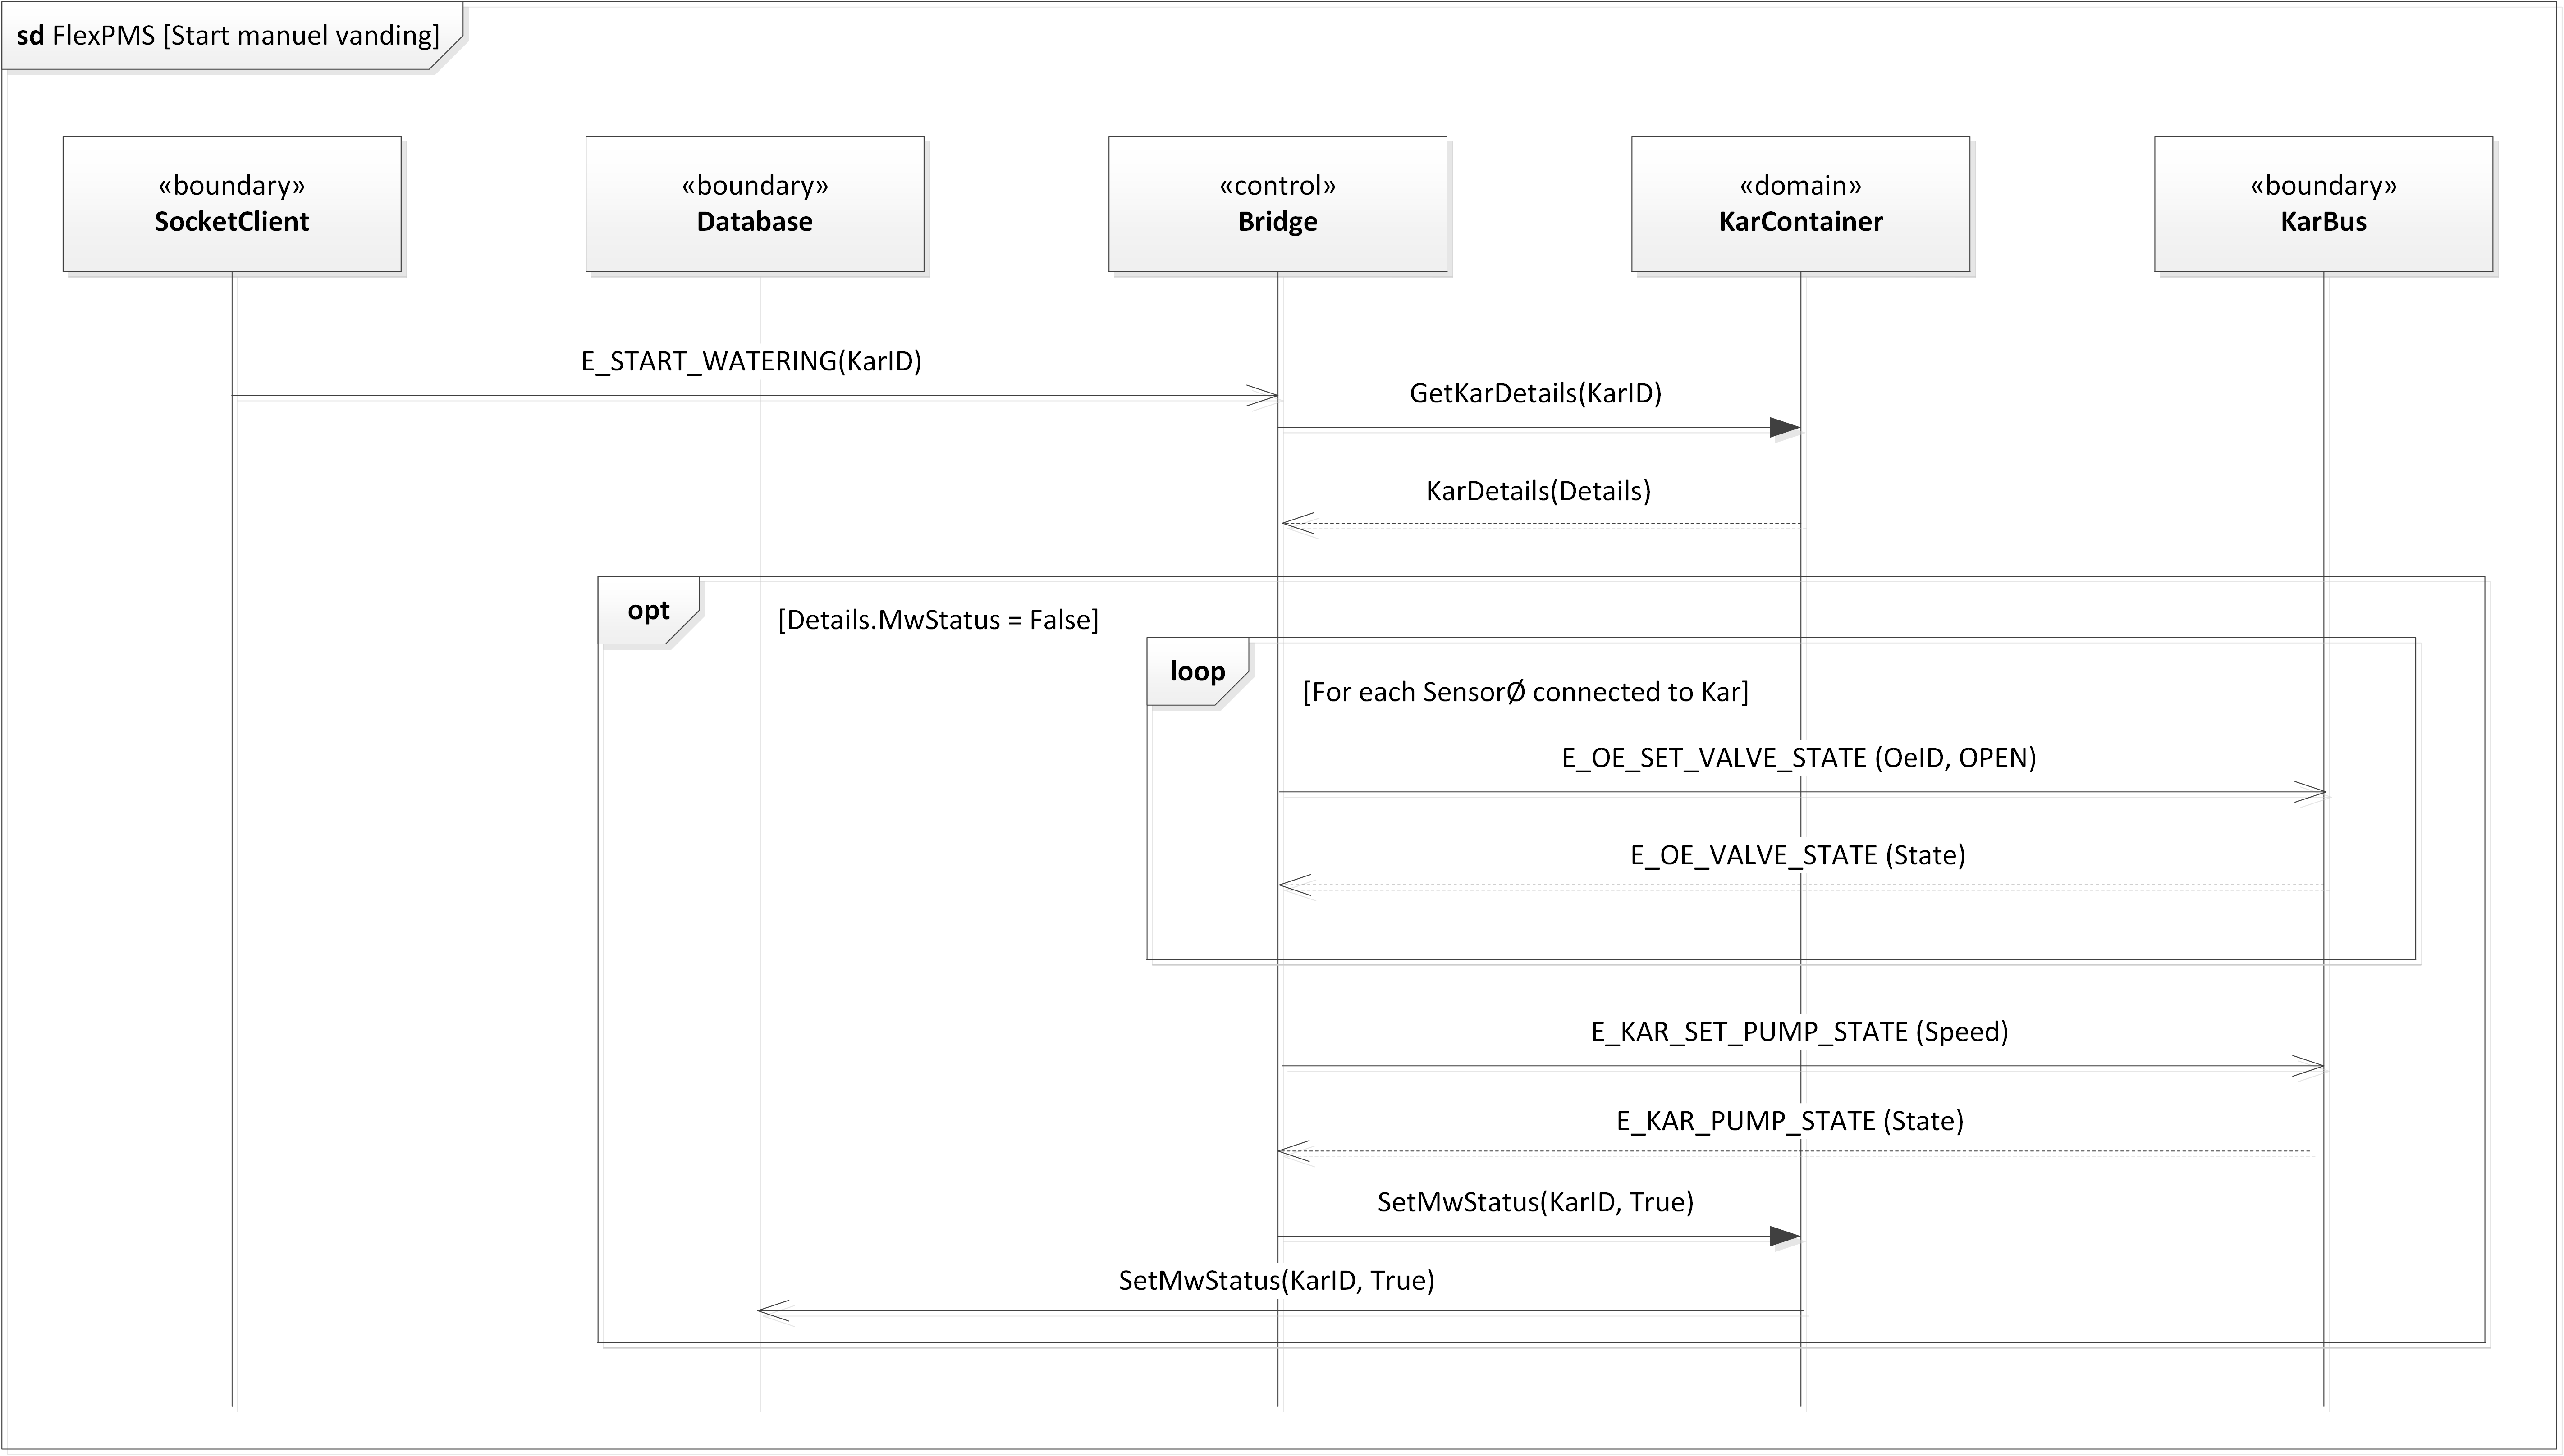
\includegraphics[scale=.6]{SoftwareArkitektur/FlexPMS/Diagrammer/Case_StartManuelVanding.png}
	\caption{FlexPMS' håndtering af at starte manuel vanding}
	\label{photo:OpenOValveUseCase}
\end{figure}


\subsubsection{Stop manuel vanding}

Når manuel vanding stoppes for et kar, så skal alle ventiler, som sidder på sensor Ø'er, der er koblet til karret, lukkes. Derefter stoppes pumpen. Herefter registreres status i databasen.

\begin{figure}[H]
	\centering
	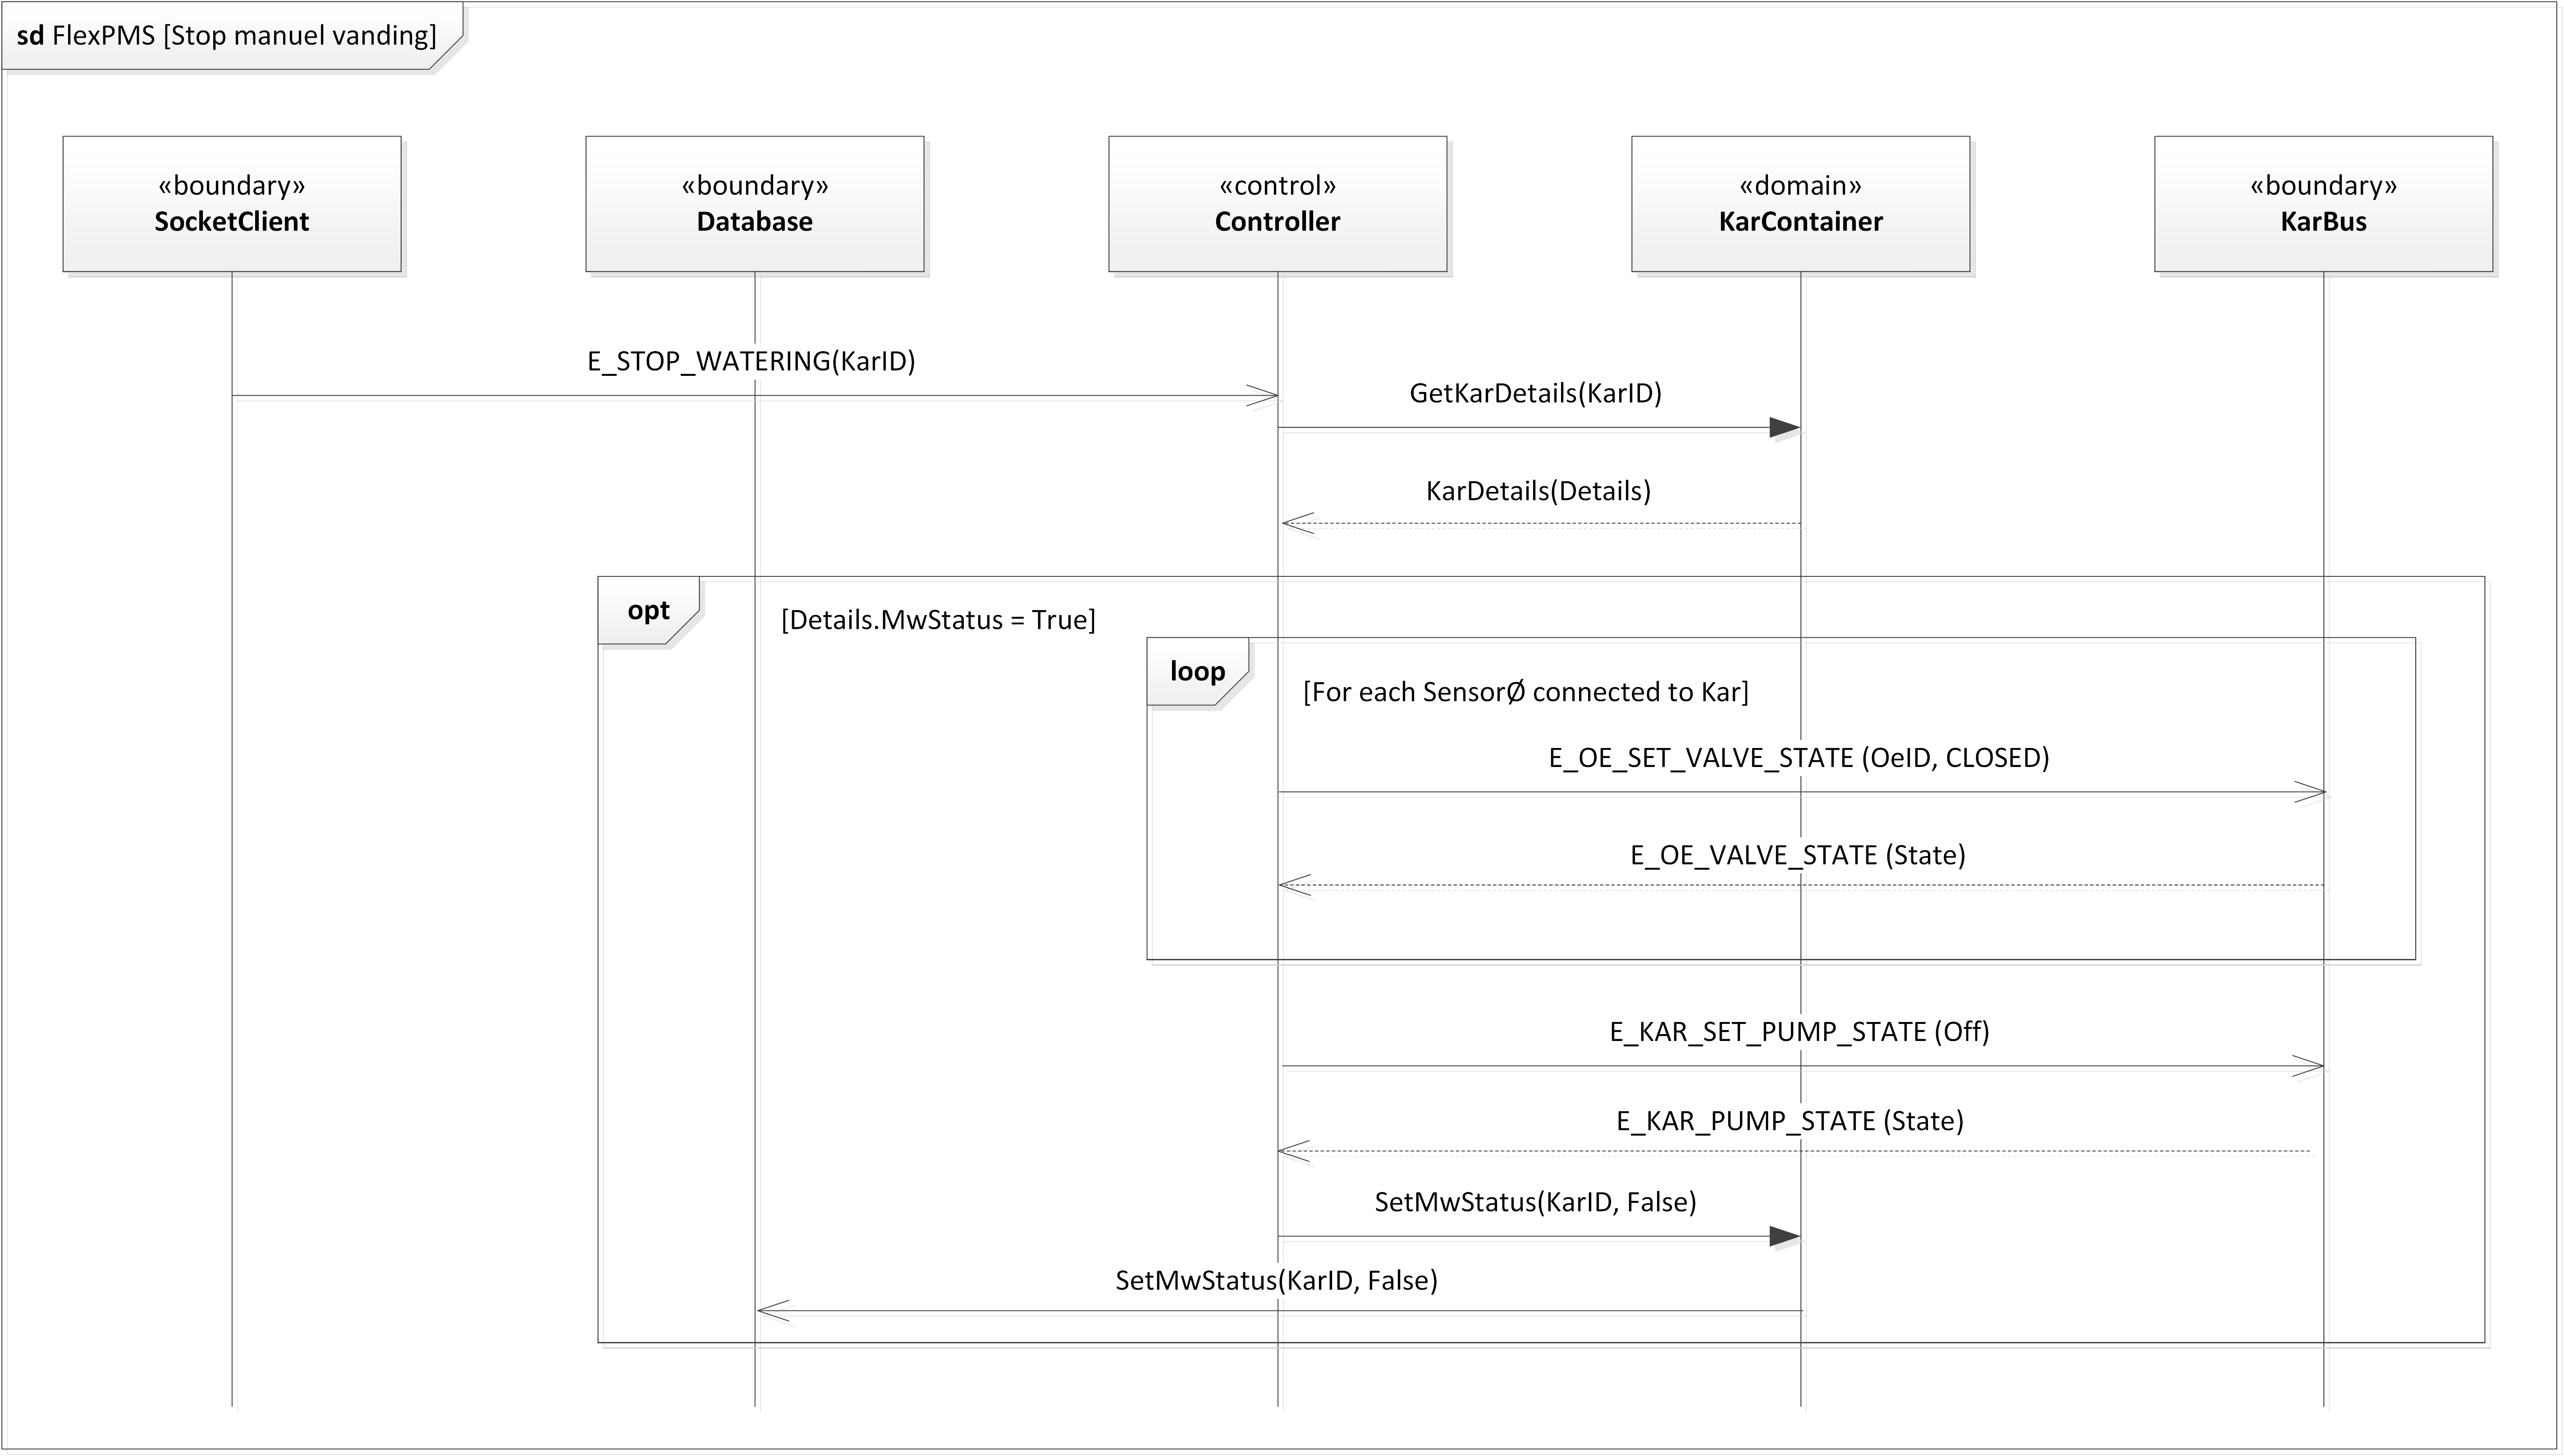
\includegraphics[scale=.6]{SoftwareArkitektur/FlexPMS/Diagrammer/Case_StopManuelVanding.png}
	\caption{FlexPMS' håndtering af at stoppe manuel vanding}
	\label{photo:OpenOValveUseCase}
\end{figure}


\subsubsection{Åben indløbsventil}

Når indløbsventilen skal åbnes, så sendes en åben-kommando til karret. Herefter registreres status i databasen.

\begin{figure}[H]
	\centering
	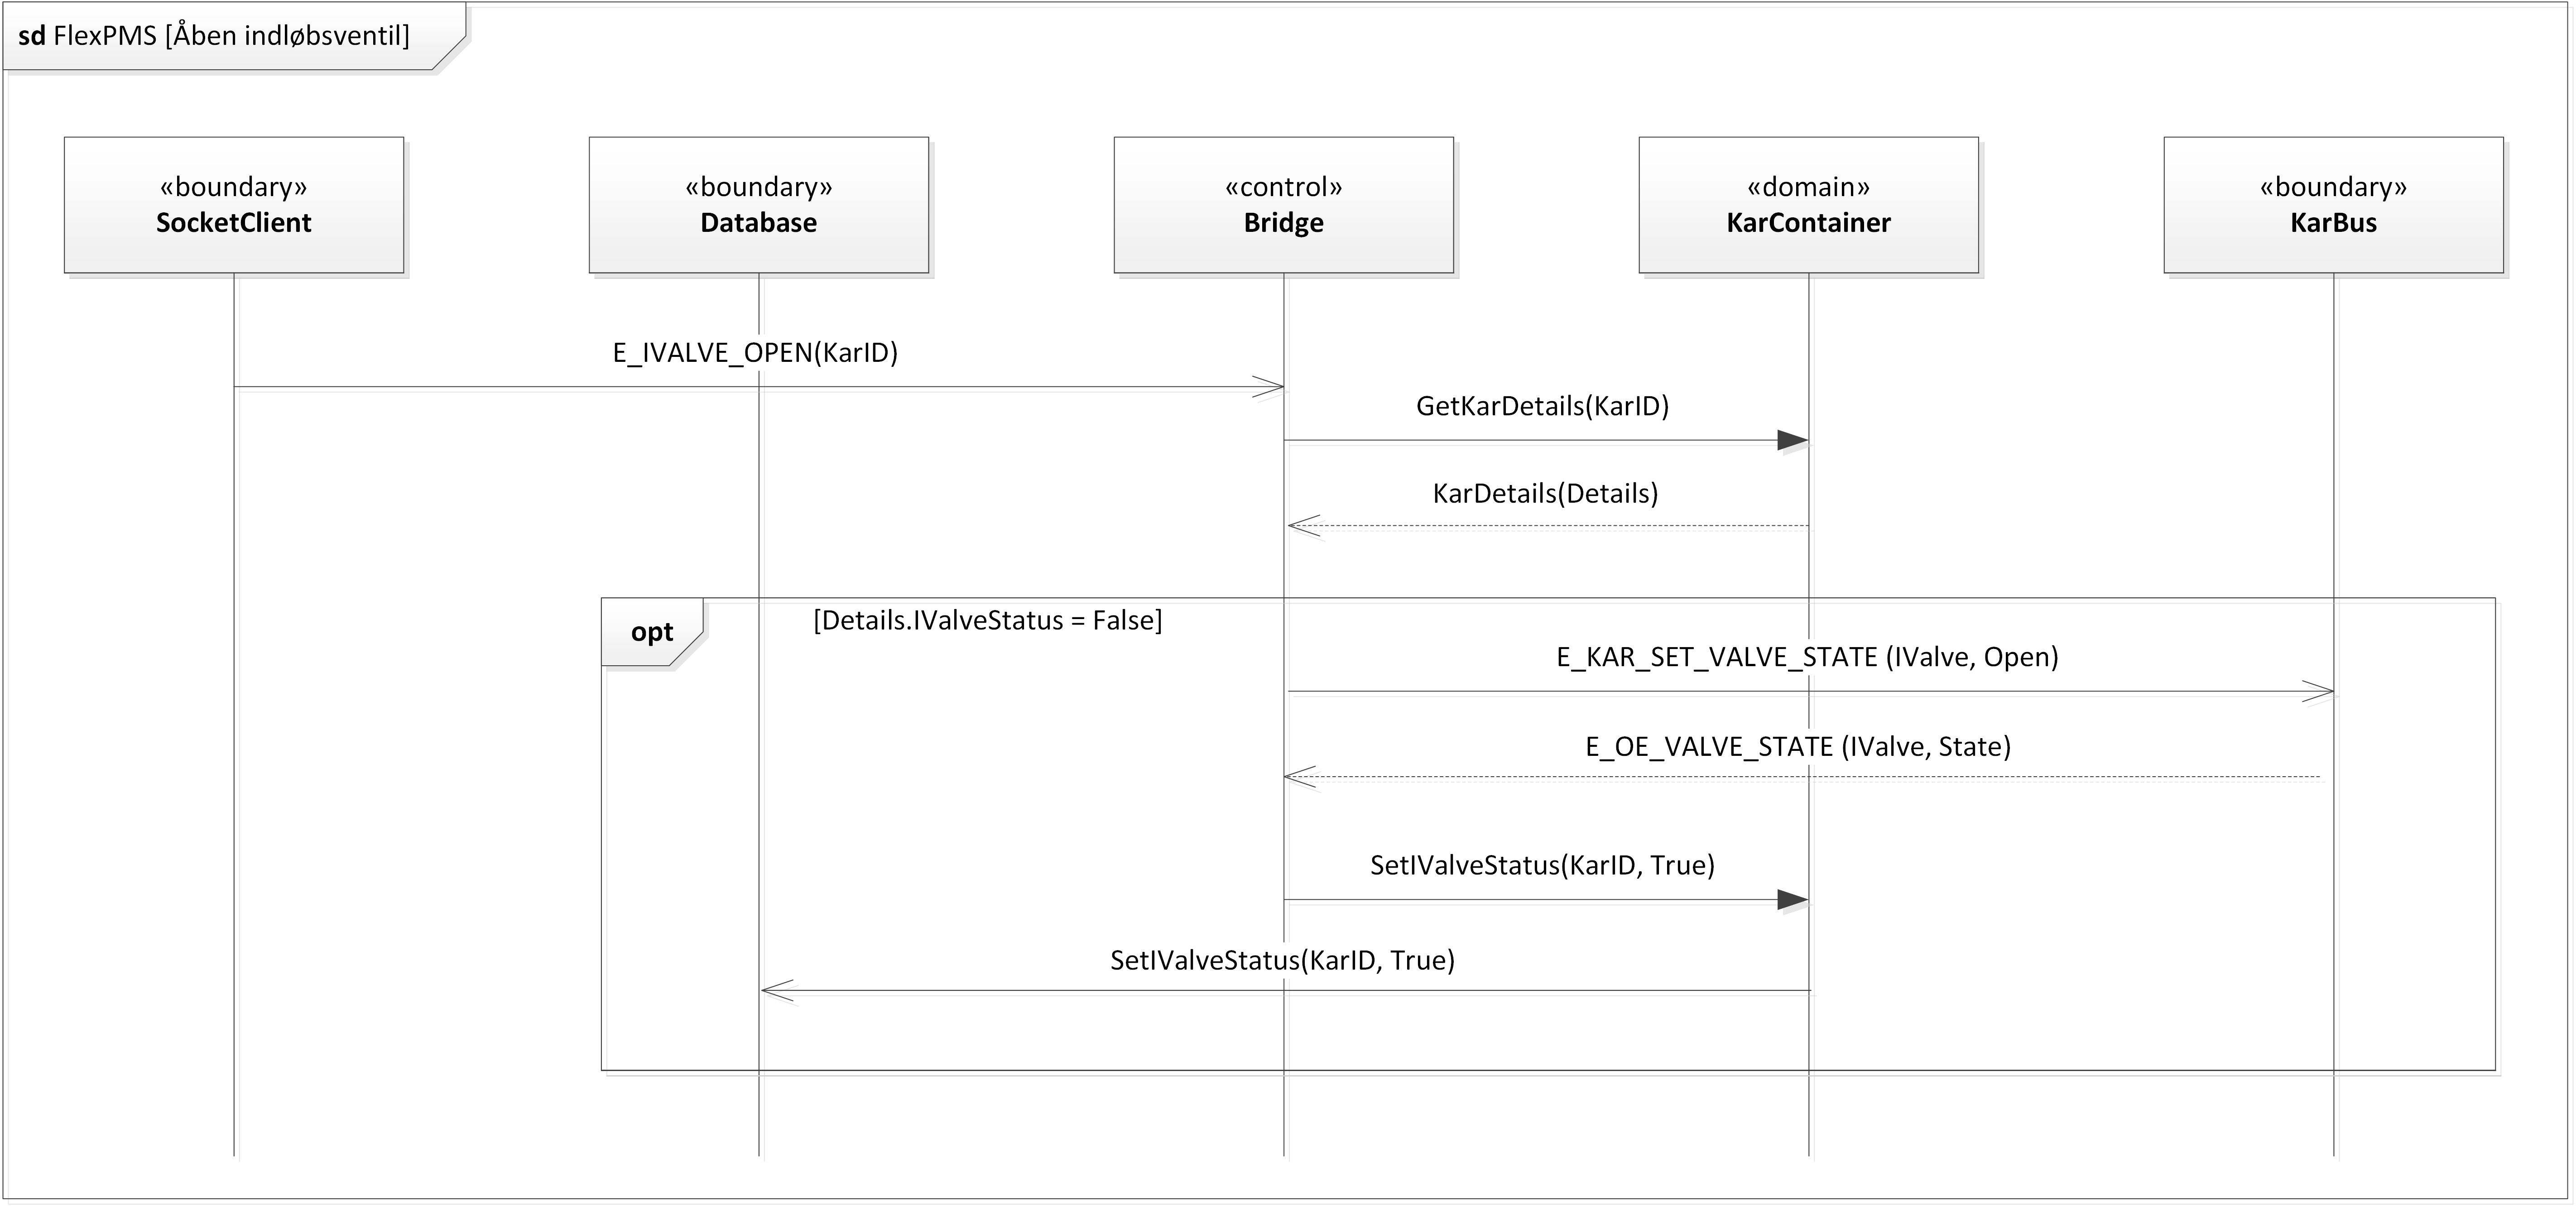
\includegraphics[scale=.6]{SoftwareArkitektur/FlexPMS/Diagrammer/Case_OpenIValve.png}
	\caption{FlexPMS' håndtering af at åbne indløbsventilen}
	\label{photo:OpenOValveUseCase}
\end{figure}


\subsubsection{Luk indløbsventil}

Når indløbsventilen skal lukkes, så sendes en luk-kommando til karret. Herefter registreres status i databasen.

\begin{figure}[H]
	\centering
	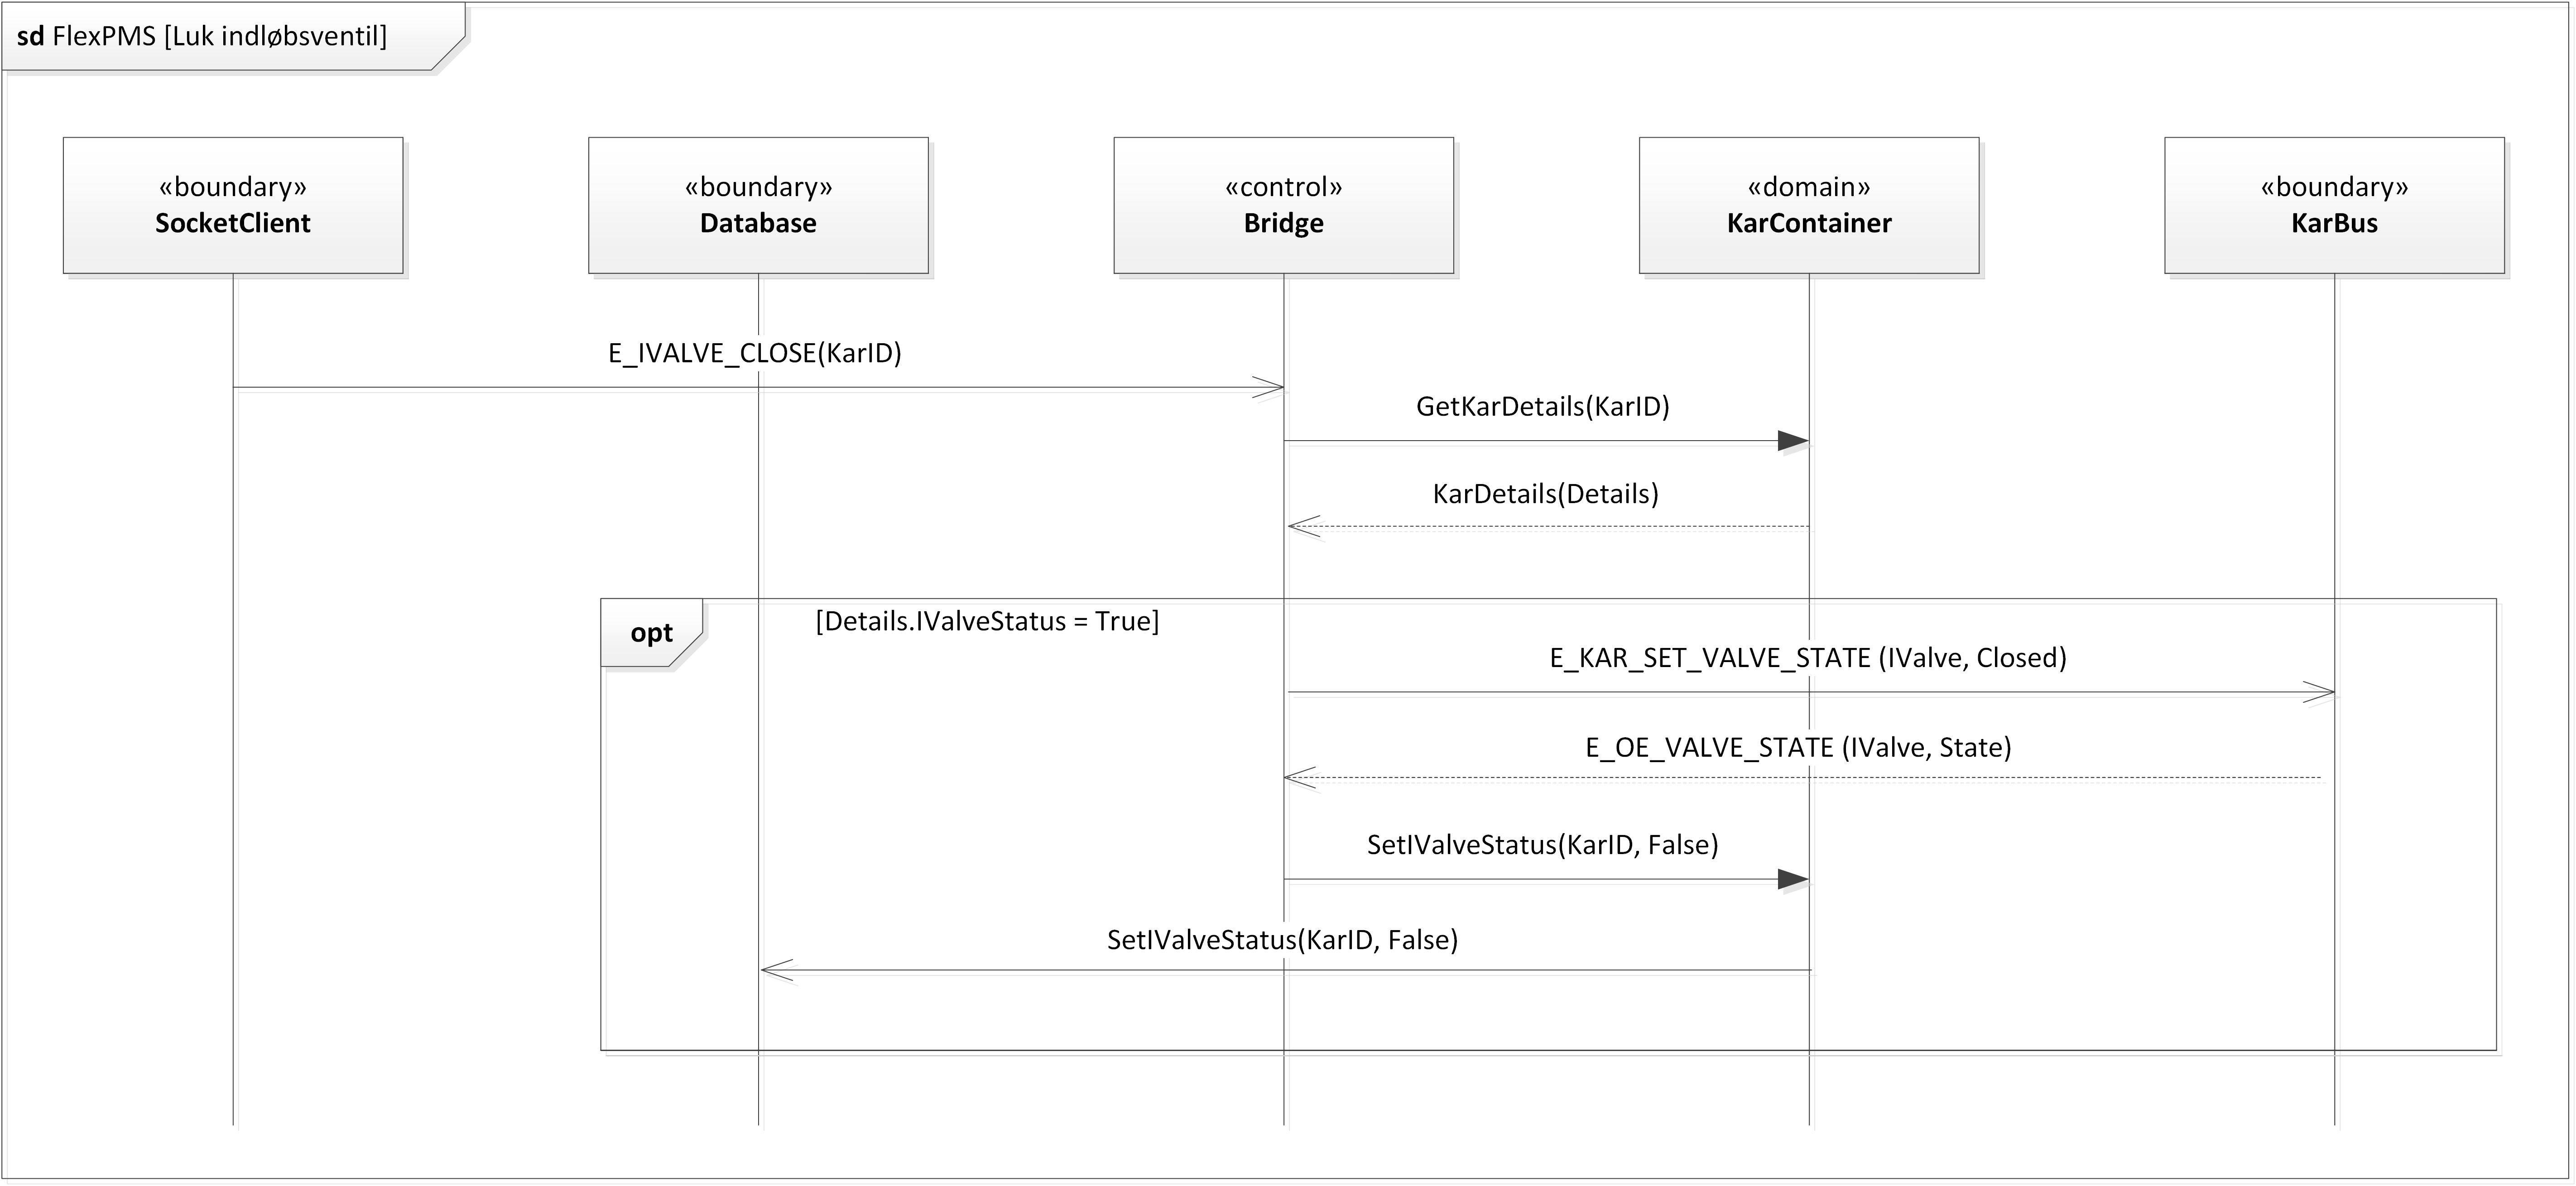
\includegraphics[scale=.6]{SoftwareArkitektur/FlexPMS/Diagrammer/Case_CloseIValve.png}
	\caption{FlexPMS' håndtering af at lukke indløbsventilen}
	\label{photo:CloseOValveUseCase}
\end{figure}


\subsubsection{Åben afløbsventil}

Når afløbsventilen skal åbnes, så sendes først en åben-kommando til karret, hvorefter pumpen tændes. Pumpen tændes fordi der skal tilstrækkeligt tryk i slangerne til, at vand kan løbe igennem ventilen. Herefter registreres status i databasen.

\begin{figure}[H]
	\centering
	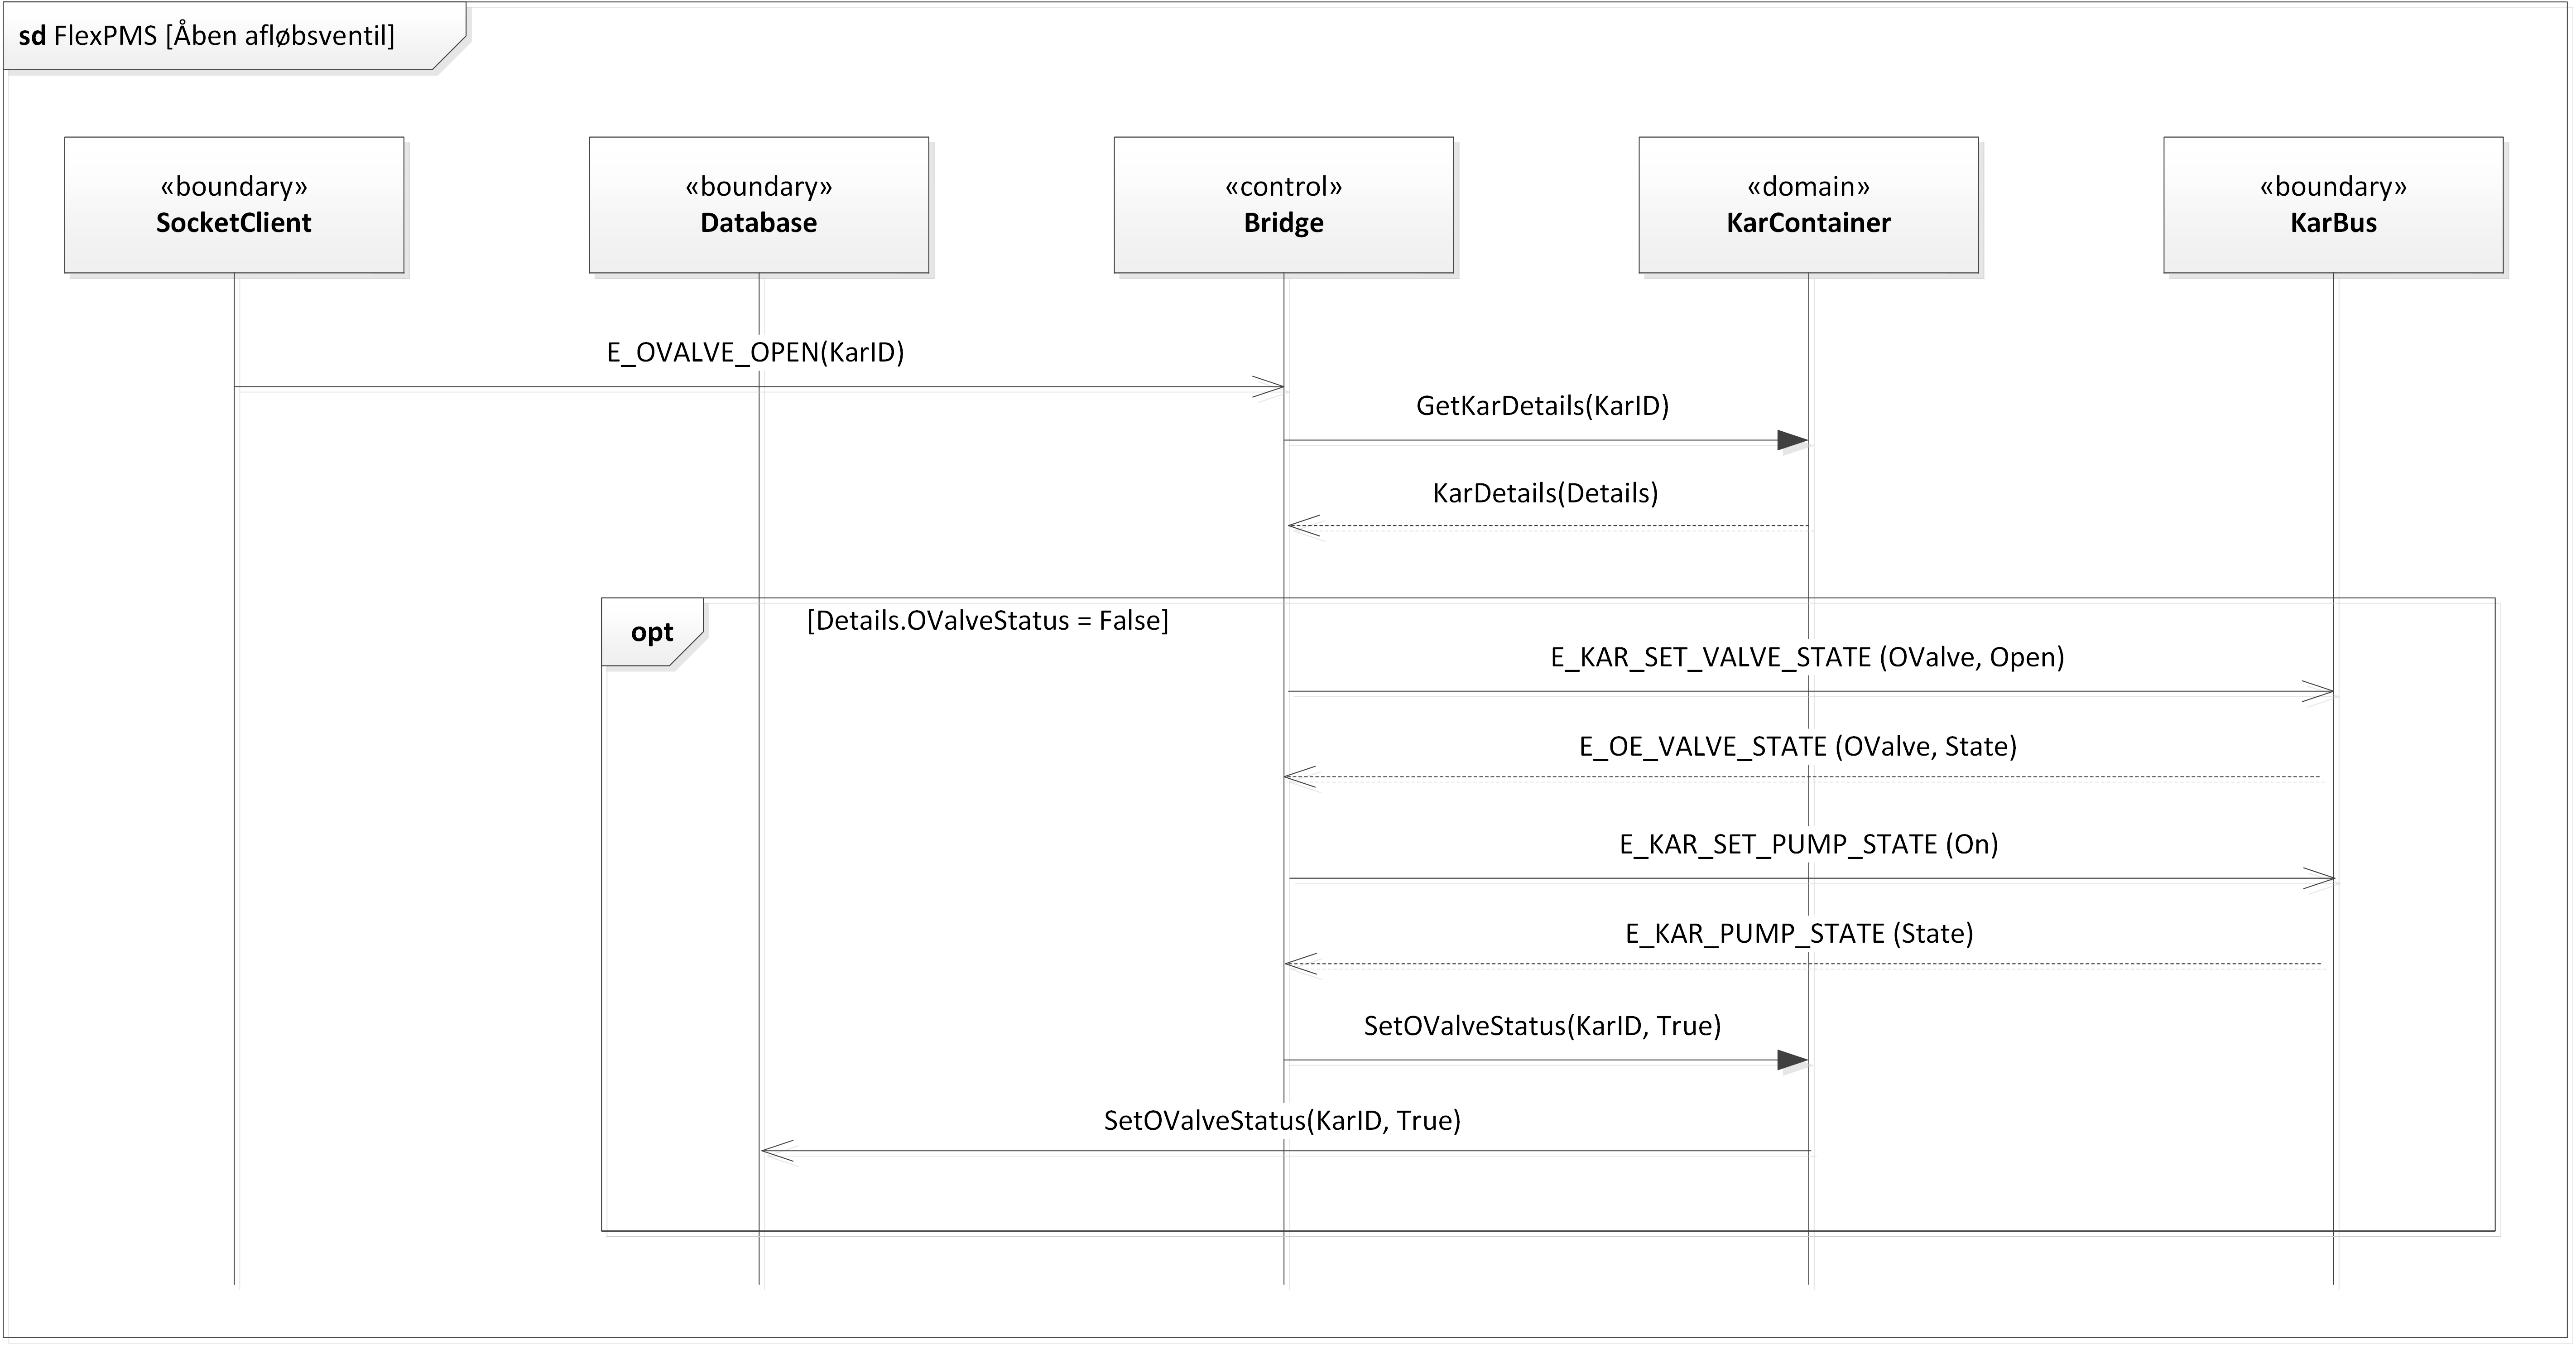
\includegraphics[scale=.6]{SoftwareArkitektur/FlexPMS/Diagrammer/Case_OpenOValve.png}
	\caption{FlexPMS' håndtering af at åbne afløbsventilen}
	\label{photo:OpenOValveUseCase}
\end{figure}


\subsubsection{Luk afløbsventil}

Når afløbsventilen skal lukkes, så sendes først en luk-kommando til karret, hvorefter pumpen stoppes. Herefter registreres status i databasen.

\begin{figure}[H]
	\centering
	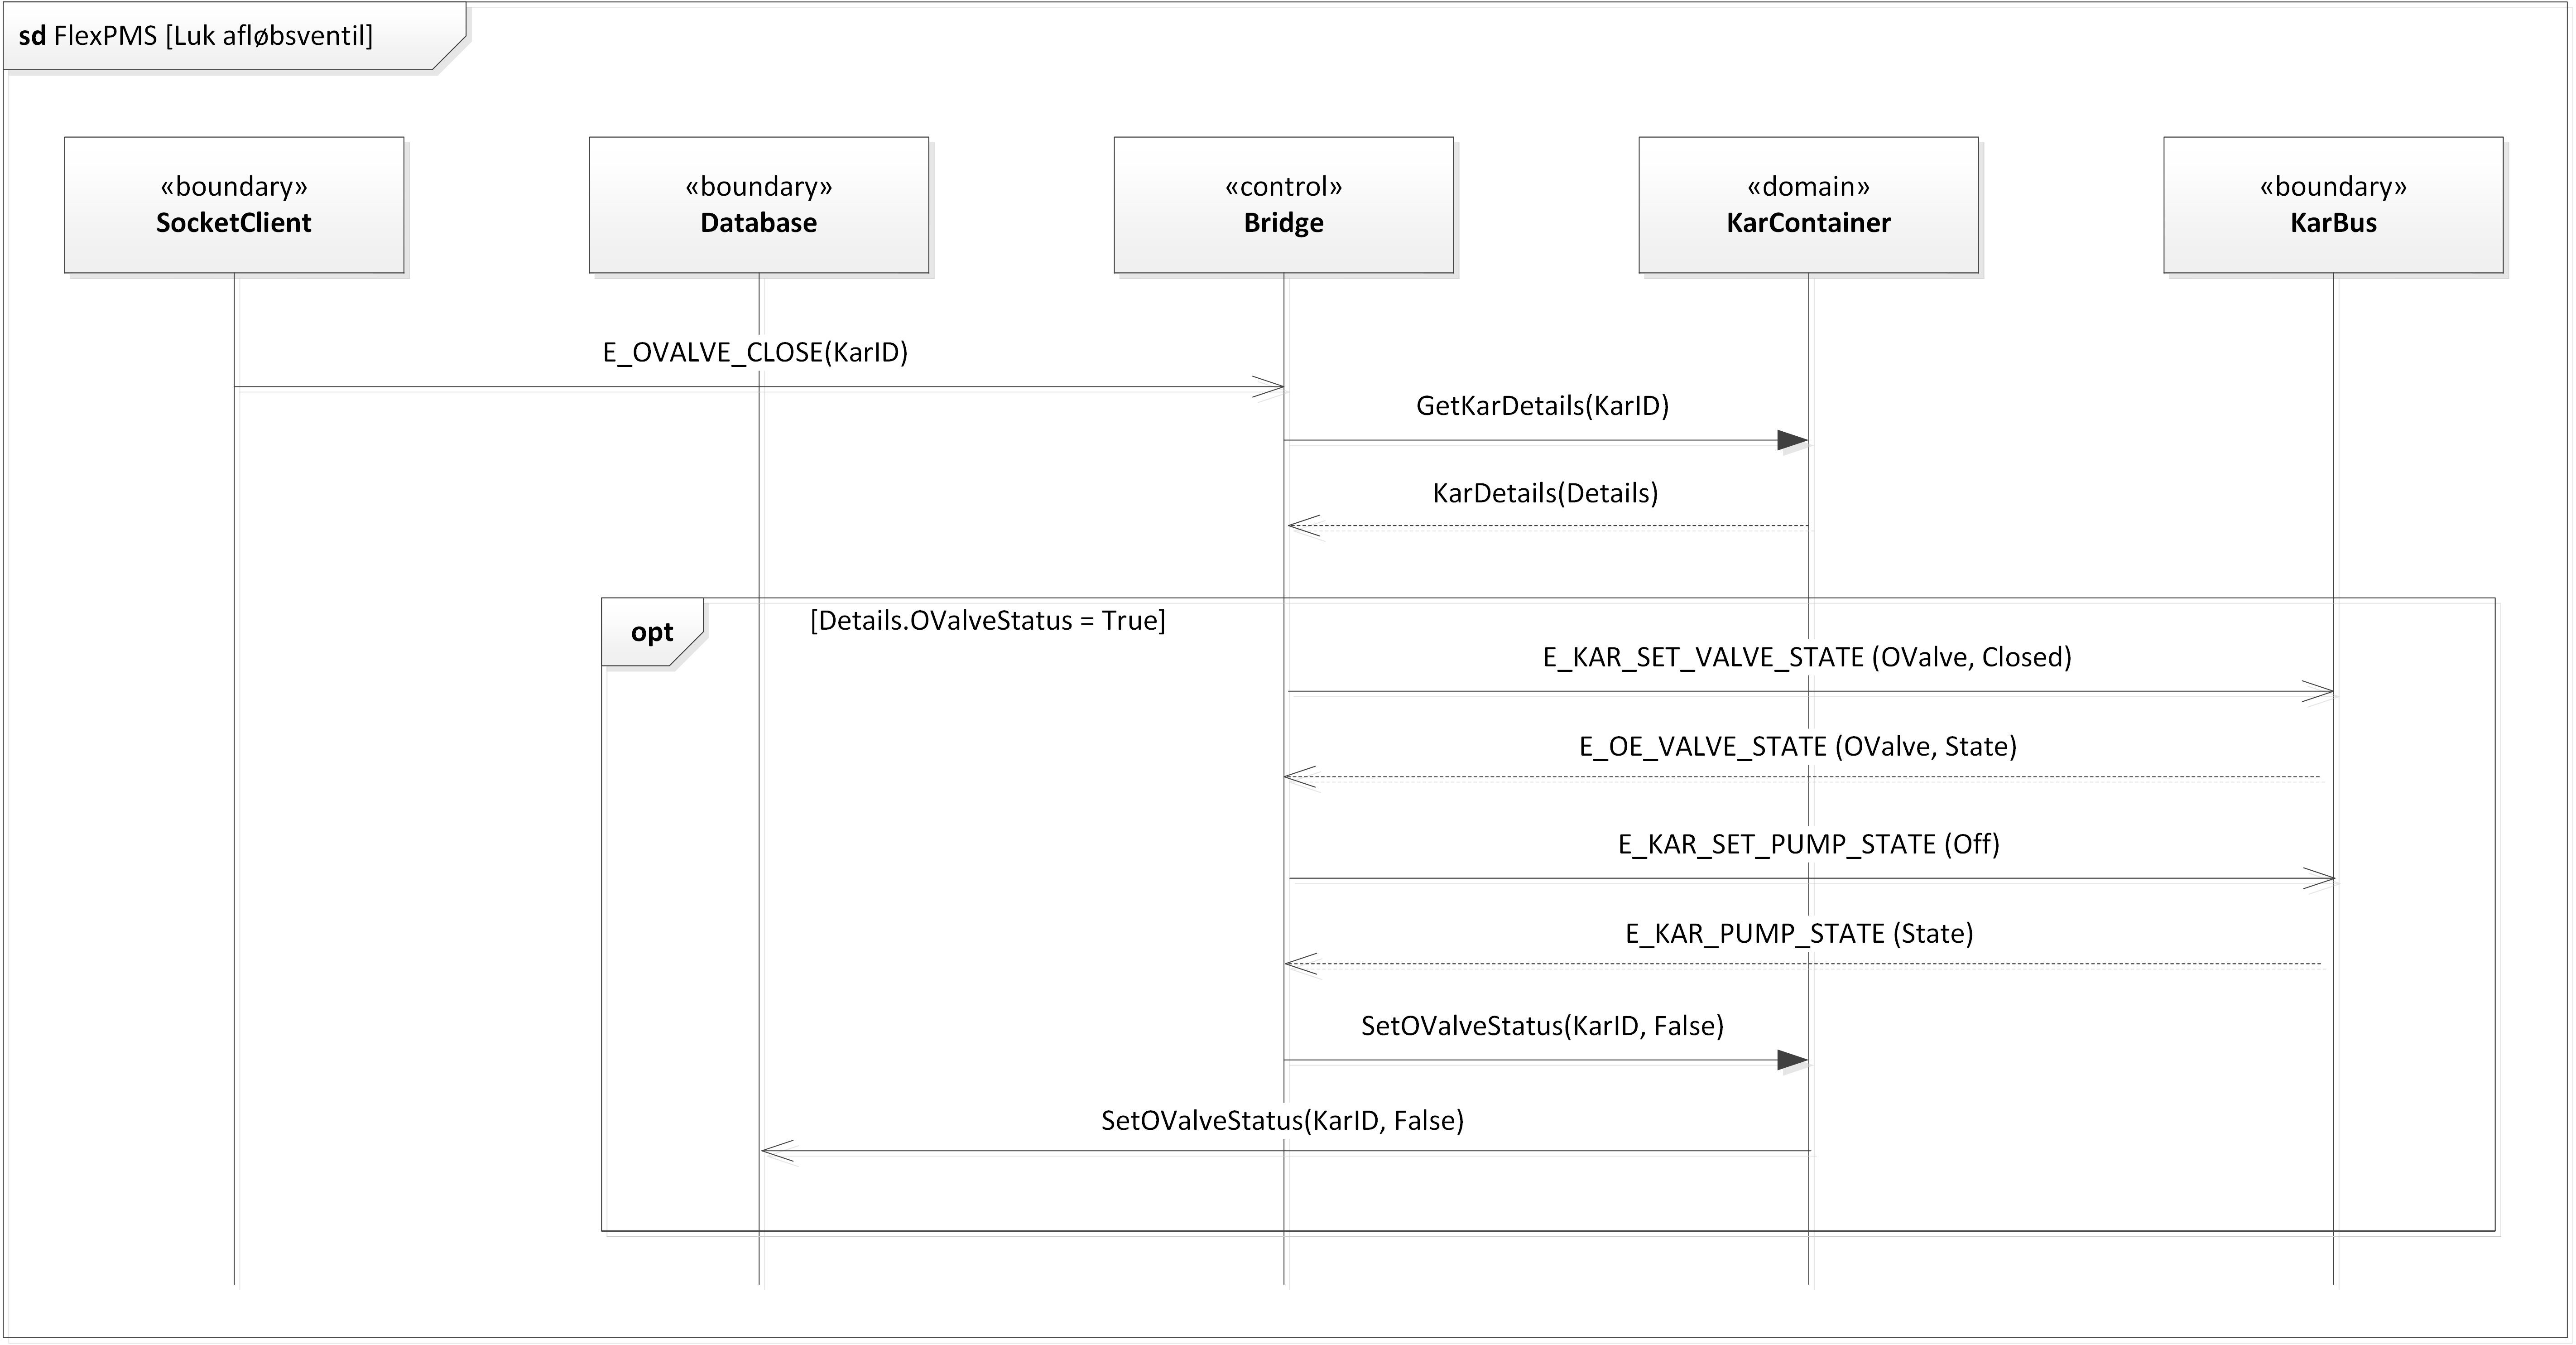
\includegraphics[scale=.6]{SoftwareArkitektur/FlexPMS/Diagrammer/Case_CloseOValve.png}
	\caption{FlexPMS' håndtering af at lukke afløbsventilen}
	\label{photo:CloseOValveUseCase}
\end{figure}

